\scanpage{318}
\mspage{17}
\[
F:X_*\longrightarrow F(X_*):\widehat{\boldsymbol\Delta}^{,o}\longrightarrow\mathrm{Ab}
\]
qui peuvent se déduire du foncteur universel
\[
\diagram{\begin{tikzcd}
\widehat{\boldsymbol\Delta}^{,o}\arrow[r,"F_o"]&(\mathrm{Ab}_*)^o
\end{tikzcd}}
\]
(défini par $(F_o)^o(X_*)=\mathbb C_*(X_*)$) en lui appliquant \unsure{l’opération} $\Omega^*$ \inserted{pour $\Omega^*\in U^L$}, ou encore qui se déduisent du foncteur cov. universel
\[
\diagram{\begin{tikzcd}[column sep=huge]
\widehat{\boldsymbol\Delta}\arrow[r,"F_o^o=(X_*\mapsto\mathbb C_*(X_*))"]&(\mathrm{Ab}_*)
\end{tikzcd}}
\]
\margin{?}
\deleted{\unsure{qui}} on dénote par $\mathbb C_*$, en lui appliquant \inserted{des} $\Omega_*$. Et les \inserted{\unsure{2}} formulations équivalentes en termes de $\Omega^\bullet,\Omega_\bullet$ opérant sur $(\mathrm{Ab}_{\unsure{\bullet|*}})^\bullet$ ($\Omega^\bullet:\mathrm{Ab}^\bullet\longrightarrow\mathrm{Ab},\ \Omega_\bullet:\mathrm{Ab}_\bullet\longrightarrow\mathrm{Ab}$), en remplaçant $\mathbb C_*(X_*)$ par $\mathbb C_\bullet(X_*)$.
\margin{Sous réserve que $L$ soit assez gros pour permettre au moins de faire des projecteurs !}

e) Quel est le rôle dans tout ceci de $\mathrm{DP}$ ? \unsure{D’un côté on trouve évident} que l’avantage de $A_\bullet$ sur $A_*$, c’est que la description d’un objet y est nettement plus simple --- on se perd facilement dans la description des op. semi-simpliciales ! --- et si on a deux notations $L_\bullet,L_*$, $L_\bullet$ est aussi nettement ``moins gros'' que $L_*$ (NB on a tjrs $L_n\subset L_{[n]}$ comme facteur direct), $L_*$ apparaît comme une sorte de version pléthorique de $L_\bullet$ !
\margin{319}

Néanmoins, dès que (dans le cas de $A=\mathrm{Ab}_{\unsure{h|k}}$ disons) $\mathrm{Ab}_{h*}$ et $\mathrm{Ab}_{h\bullet}$ sont \unsure{données} leurs structures multiplicatives --- qui ne se correspondent \uline{pas} par DP et ND --- celle de $\mathrm{Ab}_{h*}$ est plus simple à beaucoup d’égards, et s’introduit d’ailleurs de bien des façons par la suite de façon absolument impérieuse, alors que celle de $\mathrm{Ab}_{h\bullet}$ ne s’introduit pratiquement pas.
\figure{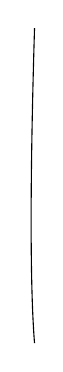
\begin{tikzpicture}\draw (0,0) .. controls (-.08,1) and (-.03,3) .. (0,4);\end{tikzpicture}}
De plus, pour les opérations tensorielles du type $\Lambda^i,\Gamma^i,\mathrm{Sym}^i$, elles manquent purement et simplement dans $\mathrm{Ab}_{h\bullet}$ (sauf de les définir par transport de structure via DP !) alors qu’elles sont \unsure{évidentes} \unsure{pour} sur $\mathrm{Ab}_{h*}$ ! Or ces structures également joueront un rôle essentiel par la suite.
